\section{Kanonische Indizierung, FIT}

Bei der kanonischen Nummerierung werden die Punkte $P(n)$ vom Ursprung ausgehend in $x$-Richtung bis zum Ende durchlaufen und aufsteigend durchnummeriert. Anschließend geht man einen Schritt in $y$-Richtung und läuft dann wieder alle Punkte in $x$-Richtung durch. Dieses Vorgehen wird solange wiederholt bis auch in $y$-Richtung das Ende des Gitters erreicht wurde. Danach macht man einen Schritt in $z$-Richtung und verfährt von dort ausgehend genauso wie zuvor schon. Damit wird erreicht das jeder Punkt im Gitter eine eigenen eindeutige Nummerierung erhält. Für die Nummerierung der Gitterkanten $L_w(n)$ ist der kleinste Punkt an dem die Kante liegt ausschlaggebend und $w$ bezeichnet die Raumrichtung in der Kante, also $x$, $y$, oder $z$.
In Abbildung \ref{fig:primal} ist diese Art der Nummerierung graphisch dargestellt wobei die Knoten in blau beschriftet sind und die Kanten in grün.
\begin{figure}[h]
	\centering
	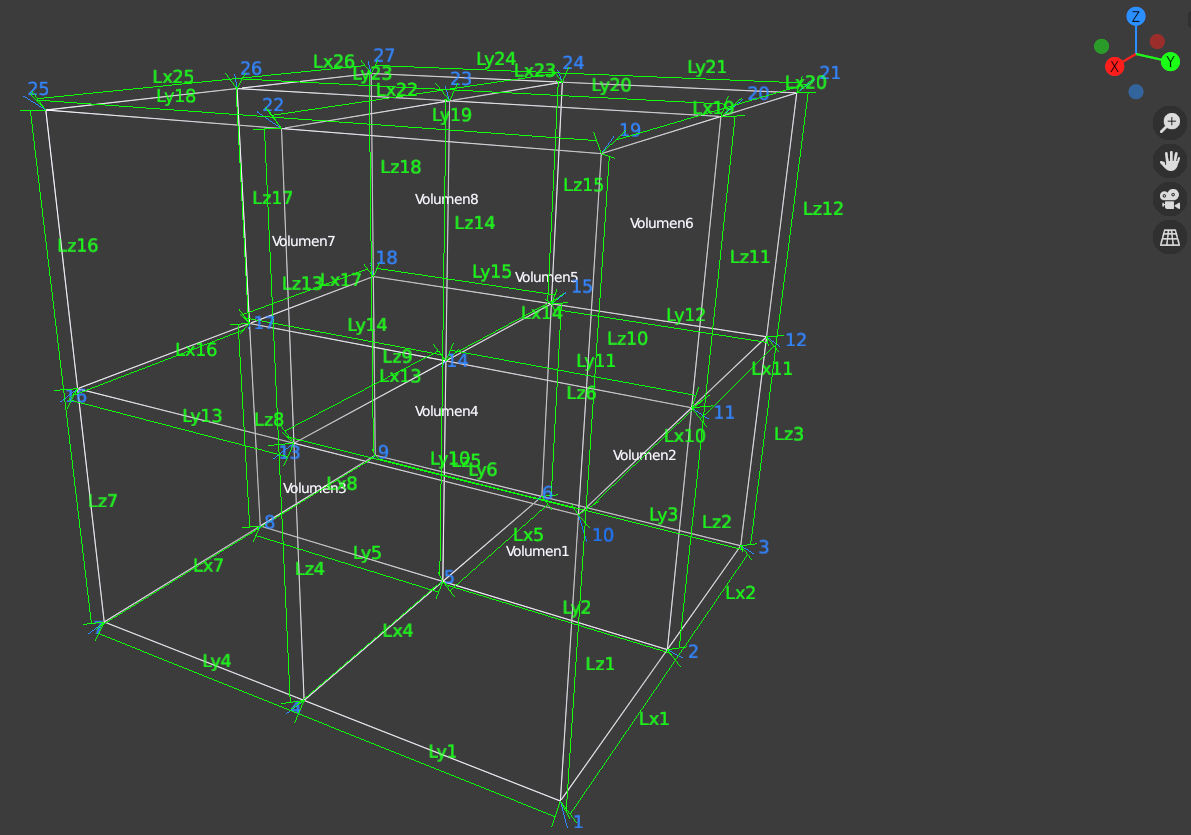
\includegraphics[width=\textwidth]{data/PrimalAllVertexAllEdge}
	\caption{Primales Gitter mit Beschrifteten Ecken und Kanten}
	\label{fig:primal}
\end{figure}

Dasselbe Vorgehen wie bei der primalen Gitterstruktur gilt nun auch für die dualen Objekte wie in Abbildung \ref{fig:dual} zu sehen ist. Dabei fällt auf dass die Nummerierung der Knoten des Dualen Gitters mit der Nummerierung der Volumen des Primalen Gitters übereinstimmen. Der Duale Knoten $\tilde{P}_1$ liegt also im Primalen Volumen $V_1$. Außerdem schneidet jede Kante des einen Gitters genau eine Fläche des anderen Gitters und auch jede Duale Zelle enthält genau einen primären Punkt. Auf diese Art zusammengehörende Objekte haben immer die gleiche Indizierung.
 
\begin{figure}[h]
	\centering
	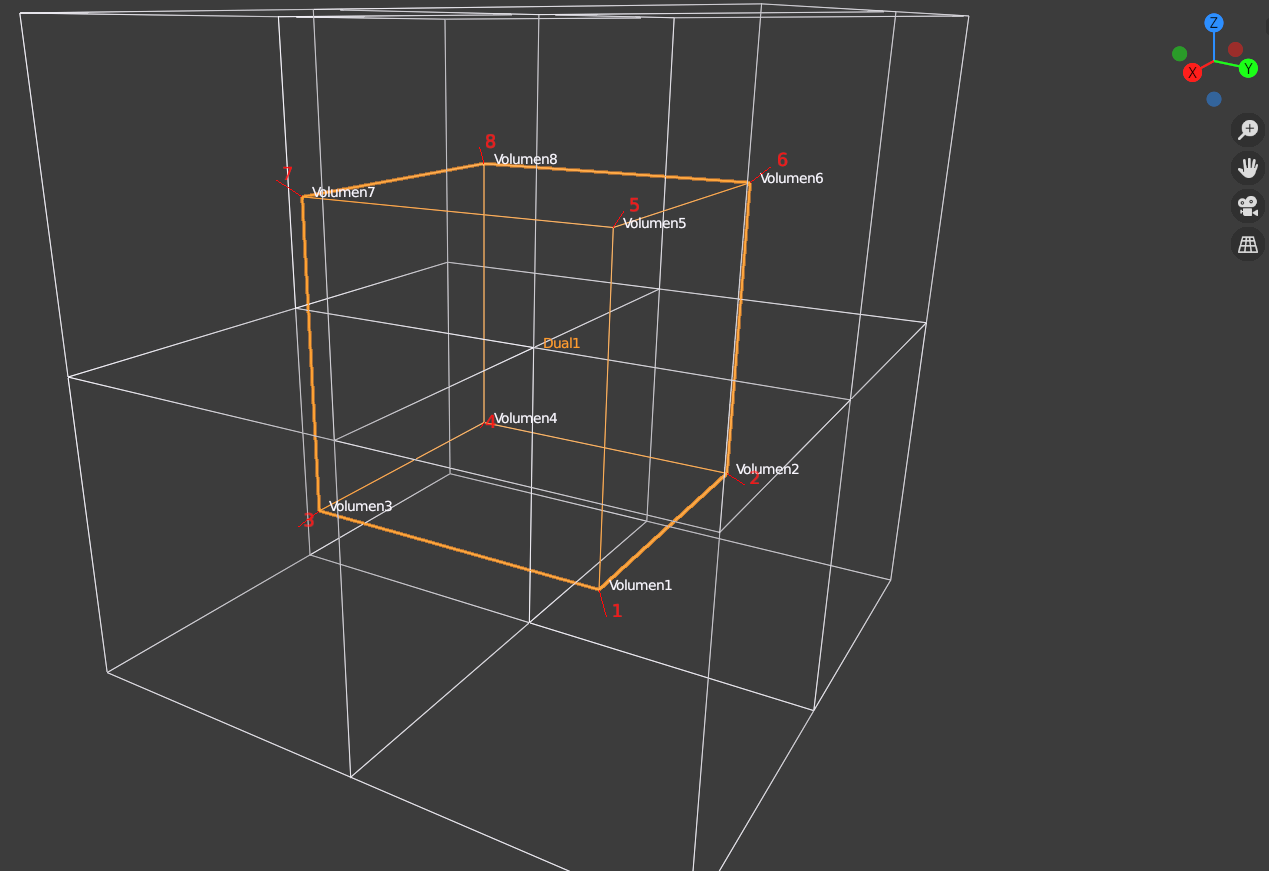
\includegraphics[width=\textwidth]{data/VolumenDualVertex}
	\caption{Primales Gitter(weiß) mit beschriftetem Dualem Gitter (orange)}
	\label{fig:dual}
\end{figure}
            	
